% Chapter 1

\chapter{Introduction to Model-Driven Development with \textsc{Cinco}}\label{ch:Basis}

This chapter lays down the fundamentals of the \acrfull{mdd} using the \textsc{Cinco} SCCE Meta Tooling Framework, as well as the steps necessary to get up and running with the framework. The term \acrshort{mdd} refers to a development paradigm where the functionalities of the software are first specified as models, from which then executable code can be automatically generated. To create and use models to represent the software system, a \acrfull{dsl} that is close to the problem domain, is needed. Application domain experts possess the knowledge of the application structure, which they represent in form of models. Domain experts and application programmers have to agree on how the specification language determines syntax and semantic of the model elements.

\section{Core Principles of Model-Driven Development}

The core principles of \acrfull{mdd} reside in the fact that software development is accelerated by providing a simple, but efficient abstraction of the software structure as a model. Those model abstraction, representation of real-world objects, are transposed trough a series of model-to-model or model-to-code transformations~\cite{stahl_et_al}. Our work is to utilize the \acrshort{dsl} provide by the \textsc{Cinco} framework to design our graphical \acrshort{dsl}, which in turn will permit the generation of a functioning \gls{Selenium} Java application.

Opposed to the common development method, applying a graphical model to layout the different user sequences allows even non-programmer (here the domain expert with much more expertise on how to design a great software documentation) to accomplish the task of documenting the features offered by the web application. Nonetheless, the programmer has the tasks --- in collaboration with the domain expert --- to specify the meaning of each model element for the code generation process.

When applied correctly, the result of the model-driven development process is a tailored application to domain. This reflects one of the main advantages of \acrshort{mdd}, the accuracy of targeting directly the specific problem. Besides, it is still possible to change the \acrshort{dsl} so that it adapts to the new challenges emerging during the development process. This can be iterated until the specification reaches preciseness wanted to solve the problem.

\section{Domain Specific Language}

A \acrfull{dsl}, as the name suggests, is a language adapted to specific development domain.~\cite{Naujokat2018} gives a succinct analogy to \acrshortpl{dsl} by saying that it is comparable to a tool specially crafted only for one specific task as opposed to general programming languages that can be seen as tools for multiple different tasks. If we stick to this analogy, just as one would start with a blueprint to construction a mechanical tool, designing as DSL required similar steps. One have to conceptually lay out the behavior and eventually --- in case it is a graphical language we want to design --- the look of each element that can be used in our DSL. 

\begin{figure}[H]
    \centering
    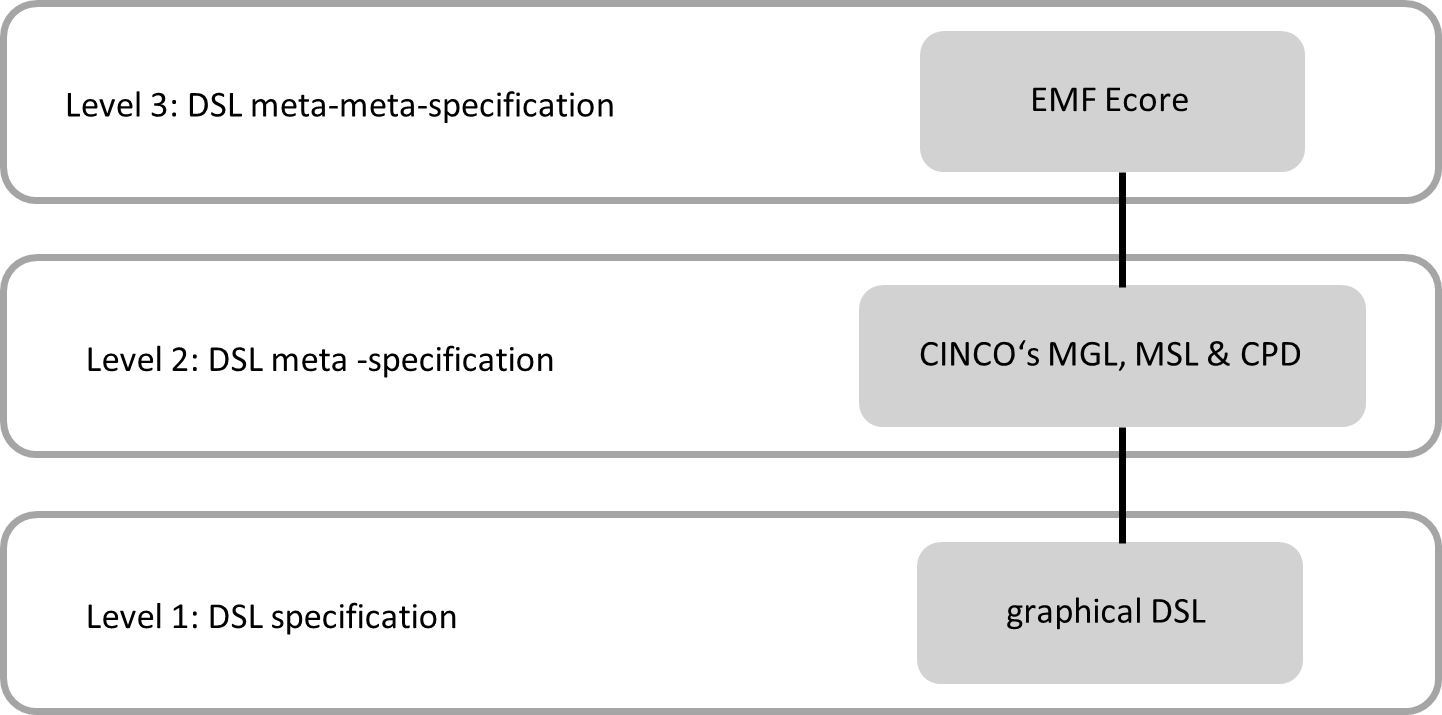
\includegraphics[width=\textwidth]{dsl_hierarchy.png}
    \caption{Hierarchy of our graphical DSL specification}
    \label{fig:modelling-hierachy}
\end{figure}

Blueprinting our DSL is equivalent to defining a meta-language or meta-DSL to our language. \textit{Meta} literally means \textit{situated behind or beyond}. So the meta-language is the descriptive language coming before our language, describing the meaning (semantic) and the relationship between the objects of our target language. In other words, the meta-DSL is the abstract syntax and the resulting DSL concrete syntax. It is possible to ascend the modelling hierarchy of meta definition until we reach a self-referencing language, like it is the case \acrfull{uml}.

In our case, we want a graphical language for creating models that represent the different parts of a web application and how the end-user can possibly interact with them. The meta-language to our graphical DSL is provided by the \textsc{Cinco} SCCE Meta Tooling framework. It comprises the \acrfull{mgl}, the \acrfull{msl} and the \acrfull{cpd} as depicted in fig.~\ref{fig:modelling-hierachy}, all has been constructed using Xtext, a language Workbench for writing textual \acrshortpl{dsl}~\cite{naujokat-diss}. Coming chapters will explain those concepts in detail.

\section{\textsc{Cinco SCCE} Meta Tooling Framework}\label{sec:cincoTool}

The \textsc{Cinco} Framework is a generator-driven development environment for domain-specific graphical modelling tools~\cite{Cinco}. It is actually developed by the chair of programming systems at the Technical University of Dortmund. One of the great features of this framework is that it allows us to generate an entire editor application with just one click from a simple textual specification language --- the \acrfull{mgl} mentioned in the previous section. 

The \acrshort{mgl} together with the \acrshort{msl} form the meta-model from which \textsc{Cinco} generates a ready-to-run modeling tools called \textsc{Cinco} product. The \acrshort{msl} is where the \textsc{Cinco} developer defines the look every node and edge element, as well as the font and color of the text to be displayed in the graphical model~\cite{naujokat-diss}. The created meta-model is based on Ecore, the meta-modeling language of the \acrfull{emf} and the Graphiti framework is used to generate the corresponding graphical model editor. Additionally, you find the right button to trigger code generation in the created editor. Chapter~\ref{ch:CP} is devoted to the \textsc{Cinco} product (the editor application), in particular section~\ref{sec:GenProcess} gives an in-depth explanation of the generation process.



\section{End-User Documentation}\label{sec:endUserDoc}

Our main goal is to produce an entire end-user documentation page on a graphical model. For that we have to first determine what the essential parts of a good documentation are. Before going further, we ought to precise that the type of documentation to be created will depend on how the documentation designer lays out the model, that means the model could be designed to represent a technical documentation, requiring deep knowledge of the application documented or it could also be structured to produce a documentation for simple end-user with no technical knowledge at all of the underlying web application.

Bearing that in mind, a good documentation should respond three important questions: \textit{what} is the purpose of the application, meaning the problem the application intends to solve, \textit{what} is the end-user supposed to do to quickly and efficiently get to the solution and \textit{how} is it achieved~\cite{5712775}. The last question is better answered by providing visual help in form of screen captures or any illustration that fastens the understanding of the documentation.

Our focus is primarily on the documentation of web application, hence documenting the \acrfull{ui}, which is composed of web elements (like buttons, navigation links, checkboxes, etc.) the end-user can interact with. This settles implicitly the type of end-user documentation we aim to create, a step-by-step guide for navigating UI to reach the expected result. 
